
\documentclass{svmult}
\usepackage{makeidx}
\usepackage{graphicx}
\usepackage{picins}
\usepackage{amssymb}
\usepackage{amsmath}
\usepackage[longnamesfirst]{natbib}
\makeindex

\begin{document}

\title*{Weight and See}
\author{
Antony Unwin\inst{1}, Heike Hofmann\inst{2}  \and Hadley Wickham\inst{2}
}
\institute{
Augsburg University, Germany \texttt{unwin@math.uni-augsburg.de}\and Iowa State University, USA \texttt{hofmann@iastate.edu}, \texttt{h.wickham@gmail.com}
}

\maketitle

\begin{abstract}
Weights are important in many areas of statistics, particularly in surveys and in model-fitting algorithms.  They are not often used in graphical displays, although it is easy to incorporate weights in most standard displays, especially area ones, and they add considerable flexibility and exploratory power.  Interpretation of weighted displays is not always easy, though difficulties in interpretation apply to all graphics.   With weighted displays the main problem arises in taking proper account of what kinds of weights are being used.

This paper discusses weighting and weighted graphical displays in general.  It describes how weighted displays can be used both statically and interactively.
\end{abstract}

\section{Introduction}
\label{intro}
Weighting in the sense of giving each case a different weight plays a role in many parts of statistics.  It is well known in surveys where different subgroups may be sampled at different rates or where adjustments need to be made for nonresponse or other reasons \citep{kish:1990}.  As \cite{hampel:1998} puts it ``Many amazing differences in bird occurrences could largely be explained by the different intensities of bird watching."  This apparently also explains away the \textit{weekend effect}, that most rare birds show up at weekends.

Weighting arises in algorithms such as in fitting generalised linear models and in smoothing.  It is also relevant for constructing indices, for meta-analysis and for methods like boosting.  In theory it can be applied in many other areas, such as clustering, but in practice that is not common.

A major issue in taking account of weighting is that there are different types of weighting and these each have to be analysed and interpreted in their own way.  There is frequency weighting, probability weighting, analytic weighting, and importance weighting.

Weighting is not commonly used in graphical displays, though often that could be very useful.  Bubbleplots are occasionally seen, that is scatterplots with each point drawn as a circle whose area depends on a third variable such as case size.  Sometimes datasets may be restructured so that what could have been drawn as a weighted plot in the original dataset can be drawn as a standard plot in the transformed version.  For instance, in the famous Berkeley discrimination dataset \citep{bickel:1975} there are $4526$ cases and three categorical variables: gender, admission and department.  There are $24$ possible combinations in all, so the data can be stored as  $24$ grouped cases with weights summing up to $4526$ or as  $4526$ individual cases.  To draw a barchart with the grouped version of the dataset, you have to use the weights and a weighted display.

Weighting leads a shadowy existence in the statistical literature.  Taking account of weighting in estimating means or proportions is technically straightforward.  The problems arise in estimating standard errors and determining distributions.  The survey literature covers this in depth for sampling weights (probability weighting, Section~\ref{pw}). Otherwise weighting only merits minor asides.  For instance, in the fascinating series of articles on representativeness in statistics by Kruskal and Mosteller at the end of the $1970$'s (\cite{kruskal1:1979}, \cite{kruskal2:1979}, \cite{kruskal3:1979} and \cite{kruskal:1980}), weighting and weights are only occasionally mentioned in connection with surveys.  Books on graphics also rarely mention weighted graphics.  There is nothing in older excellent books such as \cite{chambers:1983} or \cite{cleveland:1994}, nor in more recent fine books like \cite{Murrell:2005}, \cite{young:2006} or \cite{cook:2007}.  Even \cite{wilkinson:2005} mentions only bubbleplots and weighted graphs briefly.  \cite{unwin:2006} includes some examples of weighting, but only touches on the theory behind it.

\section{Two examples}
\label{exs}

\subsection{Family size and weighting}
\label{family}
Suppose you ask a random sample of children how many children there are in their family (the family size).  If the sample was randomly chosen from all children, then a family with nine children is $9$ times more likely to be in the sample than a family with one.  To draw a barchart showing the distribution of family size, each case should be weighted proportionally to the inverse of their family size, so a weighted barchart is needed.

On the other hand, the sample could have been randomly chosen from families with children.  In this case the standard barchart gives the distribution of family size.  Suppose, however, the distribution of the number of children living in families of size $x$ was wanted.  Then a barchart weighted by the family size would be needed, since there are $9$ children living in a family of size nine, but only one could appear in our sample.  (This weighted barchart would be the same as the standard unweighted barchart with the first sampling scheme.)

\subsection{Population structure}
\label{pop}
A thought-provoking example of the potential of weighted graphics was first given in \cite{unwin:1998a}.  The dataset contained details of the $437$ counties of the five Midwestern states (Illinois, Indiana, Michigan, Ohio, Wisconsin), including the numbers of different races living in each county.  Figure~\ref{blackhists} shows different histograms from this dataset.  The first is an unweighted histogram and shows the distribution of the percentage of blacks living in each county.  It is easily seen that most counties have low percentages of black population, but one county's population is about $40\%$ black.  The second histogram is the same data weighted by county population.  The county with the high percentage of blacks turns out to represent a large proportion of the total population (in fact, it is Cook County, where Chicago lies).  The third histogram is weighted by the black population.  Clearly this emphasises the counties with higher percentages of blacks more.  This display can be interpreted as showing how many blacks live in counties with those percentages of blacks.  Finally, the fourth histogram is weighted by the white population.  This has an opposite effect to the third one and may be interpreted as showing how many whites live in counties with those percentages of blacks.  As the majority of the population is white everywhere, the second and fourth histograms look quite similar and only differ noticeably for the higher levels of black population.

\begin{center}
      \includegraphics[width=10cm]{Blackhists.pdf}
      \caption{\label{blackhists}\em Histograms of the percentage of blacks in each county (upper left), the blacks percentage weighted by the county population (lower left), weighted by the black population (upper right), weighted by the white population (lower right).}
      \end{center}

\section{Graphics and weighting}
\label{gwts}
Graphical displays in statistics can be classified into two main groups, point plots in which each case is individually represented by a glyph (usually a point), and area plots in which groups of cases are represented by areas.  Point plots include dotplots and scatterplots, while area plots include barcharts, histograms and mosaicplots.  Boxplots are part area plot and part point plot and do not fit fully in either group.

The terminology for area plots is not consistent in the literature.  The terms barplots, barcharts, and histograms are used differently by different authors and by different software packages.  In this article barcharts are used for summarising counts of categorical or ordinal variables and have gaps between the bars, while histograms are used for summarising continuous variables and have no gaps between the bars \citep{unwin:2006}.
 
Area plots can be extended to incorporate weighting easily.  Instead of areas being proportional to the numbers of cases, they are drawn proportional to the sums of the weights of the cases.  This cannot be applied to point plots, where some attribute of the point has to be used.  One solution is to vary the size of the points and to make this proportional to the weight.  Another is to use colour or shape.  Colour has been used in displaying point densities \citep{carr:1987} as has shading \citep{hofmann:2000a} and shape has been suggested for overlapping points in scatterplots (sunflower plots in \cite{cleveland:1984}).  Pointsize is used most frequently (cf. the bubbleplots mentioned in Section~\ref{intro}), but can suffer from overlapping and obscuring of points for even a small number of cases.  It is also difficult to apply weighting for boxplots.  A possible solution is to calculate the necessary statistics as if the weights were frequency weights (cf. Section~\ref{fw}) and to draw outliers with pointsizes proportional to their weights.

\begin{center}
      \includegraphics[width=10cm]{florhists.pdf}
      \caption{\label{bubflor}\em The scatterplot on the left shows the percentage change in Bush's vote in the Florida election districts between the Presidential elections of 2000 and 2004 plotted against his percentage share in the election of 2000.  The plot on the right shows the same data with each point represented by a bubble whose area is proportional to the population of the district.}
      \end{center}
      
As always with graphics, rules are not hard and fast.  Some bubbleplots can be very informative.  The scatterplot on the left of Figure~\ref{bubflor} suggests that Bush's vote in 2004 increased more the bigger his vote share in the election of 2000.  The scatterplot on the right suggests, if anything, the opposite. 

Many statistics are plotted without weights, when the weights would contribute useful background information.  Unemployment rates and morbidity rates are often discussed by region or by population group.  Knowing the relative sizes of the regions and groups would assist in making fair comparisons.

\section{Types of weighting}
\label{types}
There are at least four different kinds of weighting that arise in data analyses.  This is not always apparent in software packages, though the Stata software does a nice job of handling all four and its documentation provides clear definitions \citep{stata:2007}.  The following hypothetical example will be used in this section to illustrate all four weightings on the same dataset.  Its structure is similar to that of international surveys such as the European Social Survey (http://ess.nsd.uib.no/).  There are $M$ groups with populations
$$N_j\qquad \text{ where }\qquad j=1,\dots,M\qquad\text{ and }\qquad \sum_{j=1}^MN_j=N.$$
Simple random samples are taken from each group of sizes
$$n_j\qquad\text{ where }\qquad j=1,\dots,M\qquad\text{ and }\qquad \sum_{j=1}^Mn_j=n.$$
Each person $i$ sampled from group $j$ is checked to see if they are ill or healthy.
\[
Z_{ij}=\begin{cases}
  1    & \text{if ill}, \\
  0    & \text{if healthy},
\end{cases}
\text{ with } i=1,\dots,n_j \text{ and } j=1,\dots,M
\]

\subsection{Frequency weighting}
\label{fw}
The simplest kind of weighting is frequency weighting (FW) as in the example at the end of Section~\ref{intro}.  If all attribute values for a group of $m$ cases take the same values, then the data can be stored as a single case with a frequency weight $m$.  The dataset from the hypothetical example can be written with at most $2M$ entries (combinations which do not occur need not be included). Let $m_{kj}$ denote the number of persons in group $j$ with health $k$, i.e. $m_{kj} = \sum_{i=1}^{n_j} \left( Z_{ij} = k \right)$, then the data set can be written in the form
$$(k,j, m_{kj}) \quad \text{ where } k\in\{0,1\}\quad\text{and}\quad j=1,\dots,M.$$
The values $m_{kj}$ are then frequency weights:
$$w_{kj}^{FW}=m_{kj}\quad \mbox{ with } m_{0j}+m_{1j}=n_j$$

Frequency  weights reflect multiple independent individuals with the same values.  These weights are always nonnegative integers.  Assuming the independence of observations, frequency weights are just a computational convenience and cause no problems of interpretation.  For frequency weights the $\ell$th set of cases has
$$w_\ell^{FW}=m_\ell \qquad \mbox{ and }\qquad \sum_\ell m_\ell = n$$
where $n$ is the total number of sampled cases.  The Berkeley discrimination dataset mentioned in Section~\ref{intro} uses frequency weights.

\subsection{Probability weighting}
\label{pw}
Probability weighting (PW) arises in sampling whenever a non-random sampling scheme is used.   There are e.g. occasions when it is efficient to sample small groups more than larger ones.  When results are combined, the weighting used for a case is the inverse of the probability of that case being sampled.  In the hypothetical example, the dataset $\{Z_{ij}\}$ with $i=1,\dots,n_j$ and $ j=1,\dots,M$ has $n$ entries and probability weights that are inversely proportional to their sampling probability:
$$w_{ij}^{PW} \propto \frac{1}{n_j/N_j}=\frac{N_j}{n_j}$$
The PISA Study \citep{adams:2002}  used a complicated multilevel system of sampling to facilitate comparability of results across schools and countries.  The weight $W_{ij}$ for a student $i$ in school $j$ was made up of two base weights (one reflecting the selection of school and one reflecting the selection of the student within the school) and $5$ (five!) adjustment factors.  Sophisticated weighting may be fair, but it is not always transparent.
\par
Probability weighting can also arise for other reasons, for instance to adjust for non response between groups.  A probability weight reflects the size of group that an independent individual represents in sampled data.  If individual $i$ has probability $p_i$ of appearing in the sample, then his weight
$$w_i^{PW} \propto 1/p_i$$
The weights may be normalised so that they sum to $1$ or to an `equivalent sample size' $n$.  Probability weighting was used in the examples in Section~\ref{family}.

\subsection{Analytic weighting}
\label{aw}
Analytic weighting (AW) is necessary when results from different samples are combined and plays a critical role in metanalysis.  The samples may be measured with different precision and so weights equal to the inverse of the variance are used.  This means that observations measured with higher precision get more weight.
Returning to the hypothetical example, consider a dataset of illness rates $r_j$ by subpopulation, i.e. 
$$\left\{r_j=\frac{\sum_{i=1}^{n_j}Z_{ij}}{n_j}\quad \text{ for }j=1,\dots,M\right\}.$$

Analytic weights are almost always based on an underlying model. The underlying model, here is assuming binomially distributed random variables $Z_{.j} \sim B_{n_j, p_j}$, which induce for the rates $r_j$ analytic weights that are inversely proportional to their variance:
\[
w_j^{AW}(r_j) \propto \frac{n_j}{r_j(1-r_j)}.
\]
We have assumed $N_j>>n_j$ so that there is no need to correct for finite sampling.
 
If the measurement variances are equal, but there are more observations in one sample than in another, then analytic weighting is equivalent to frequency weighting (weighting by the number of observations), when you are estimating a mean or proportion.  For example, assuming $r_j\approx r$ for all $j$ leads to
$$w_j^{AW} \propto n_j=w_j^{PW}$$
In general the statistic from the $j$th group has weight
$$w_j^{AW} \propto \frac{n_j}{\sigma^2_j}$$

Adding precisions (inverse variances) is well-known in Bayesian modelling.  Taking a sample from a normal distribution, whose mean has an a priori normal distribution, leads to a normal a posteriori distribution whose precision is the sum of the other two precisions.

Graphics associated with analytic weighting often use the square root of the inverse of the weight.  Scientists commonly plot their points with confidence intervals around them (or other intervals, sometimes you have to read the small print to be certain what exactly is being displayed).  Points with high uncertainty and hence low weight have bigger intervals and take up more of the display, the opposite of what weighting means in the kinds of displays using weights discussed here.

\subsection{Importance weighting}
\label{iw}
Importance weighting (IW) is used when cases are judged to have different importance.  Company data might be weighted by the size of the company in turnover or market capitalisation, illness rates for different ages and genders would be weighted by the relative sizes of the groups, market share changes by product market shares, product prices by numbers of units sold or turnover.  As these examples (and the examples in Section~\ref{pop}) show, there can be a wide choice of possible weighting variables when using importance weighting.

Shopping panel data includes information on whether someone bought a product and how much they bought of it.  The quantity bought by someone is an importance weight and not a frequency weight.  One person buying two units of a product is statistically different from two people independently buying one unit each.

In the illustrative example, the dataset $\left\{r_j=\frac{\sum_{i=1}^{n_j}Z_{ij}}{n_j}\right\}$ has importance weights 
$$w^{IW}(r_j)=N_j$$
In this case it is interesting to note that
$$\sum_{i=1}^{n_j}w_{ij}^{PW} \cdot  n_j \propto  w^{IW}(r_j)$$
Importance weights are equal to the sum of probability weights when importance is measured by equivalent units that may be regarded as independent.  This will not generally hold for importance weights in practice.

The example can be extended to show another kind of importance weighting.  Suppose that those being questioned are actually part of a clinical trial and are also asked about a range of possible side-effects.  A weighting is associated with each side-effect according to its seriousness.   Side-effect weights can then be added for each patient to produce a weighted measure of the overall unwanted consequences of the treatments.

Note that the so-called importance sampling weights that are used in bootstrapping and elsewhere are examples of probability weights not of importance weights.

In general the $i$th case has weight
$$w_i^{IW}\propto N_i$$

\subsection{Other kinds of weighting}
\label{otherw}
Where weighting is used in iterative algorithms such as model-fitting and smoothing, the weights attached to each case vary during the procedure.  It would be informative to plot the weights and to observe the changes over the iterations.  This is more a computational issue than a statistical one and is not pursued further here.

Density estimation can also be said to use weighting.  Each point is distributed across a range of values, rather than being included in analyses with a single weight.  The weight distribution depends on the density estimation model used.

Geographic weighting is used in spatial smoothing and calculating local statistics (\cite{unwin:1998b} and \cite{brunsdon:2007}).  Cases, often regions, do not have a single weight attached to them.  Their influence (weight) on each other case is calculated individually and depends on the form used to model spatial closeness and on the influences of the other cases in those neighbourhoods.  Surprisingly, only distance or adjacency is incorporated in the weights, not size or any other measure of importance.

\subsection{Properties of weights}
\label{props}
Weights have to be additive and nonnegative and should not include any missing values.  The additive property is clear and rules out percentages (so the histogram in Section~\ref{pop} cannot be weighted by the percentage of whites, only by numbers of whites).  The need for non-negativity is not so obvious, as some displays can be drawn with negative values (e.g., a modified barchart or scatterplots using colour rather than size to express weight).  However, in general this does not work.  It is certainly inappropriate for interactive graphics, cf. Section~\ref{ig}, where a combination of two cases with equal and opposite weights in a display would give an area of $0$ and neither case could be highlighted on its own.  It is safer (and more understandable for users) to insist on non-negativity.  If a weight variable includes missing values, then the corresponding cases will not be plotted.  This can mislead.  \cite{unwin:1996} describes how missing values can be taken account of in many standard graphics to avoid misleading interpretations.  These ideas have been implemented in the software packages MANET \citep{hofmann:2000a} and Mondrian \citep{theus:2002}.  Tools for dealing with missing values in weights do not yet exist.

Apart from technical restrictions on weights, there are also intepretative restrictions.  Many combinations just do not make much sense.   Weighting product prices by units sold or by turnover is fine.  Weighting the product prices by total weight of product sold can be interesting (e.g., for chocolate bars), though not always (e.g, for computers).  Each case needs to be considered carefully to ensure that the resulting plot is interpretable in a reasonable way.

\section{Interactive graphics and weighted displays}
\label{ig}
For all area plots case-based linking works as it always does, though with highlighting being proportional to weights instead of to counts.  For point plots linking is possible if glyph size is used to represent weights, but even then highlighting is problematic due to overlapping in all but the smallest of datasets.  If colour or shape is used to represent weight, then highlighting becomes more difficult still.

Examples of interactive graphics with weighted displays are given in Figures~\ref{webwords1} and \ref{webwords2}.  The dataset contains information on how often each day words on a website are viewed (number of page impressions), clicked on, and lead to sales.  The period covered is the first eight months of 2006.  The histogram on the left of Figures~\ref{webwords1} is of weeks weighted by numbers of page impressions.  One of the advertising keywords has been selected to give the histogram on the right.  It is clear that the decline in page impressions for this keyword is one of the reasons for the overall decline.

\begin{center}
      \includegraphics[width=12cm]{WebWords1.pdf}
      \caption{\label{webwords1}\em Histograms of weeks weighted by page impressions.  For the plot on the right, one of the keywords has been selected from a barchart (not shown).}
      \end{center}

Figures~\ref{webwords2} shows on the left a histogram of weeks weighted by clicks.  The decline in page impressions had little or no effect on the numbers of clicks observed.  In the spinogram on the right, the keyword corresponding to the name of the company has been selected.  It can be seen that the percentage of these clicks remains constant across the period.

\begin{center}
      \includegraphics[width=12cm]{WebWords2.pdf}
      \caption{\label{webwords2}\em On the left is a histogram of weeks weighted by clicks and on the right the corresponding spinogram with keyword of the company's name selected.}
      \end{center}


\section{Weighting in multivariate graphics}
\label{mv}
Figure~\ref{bubflor} shows a bivariate example of a weighted plot.  Parallel coordinate plots are effective for displaying unweighted multivariate continuous data and can in principle be enhanced to cope with weights by drawing the points as circles with areas proportional to weights and the lines with widths proportional.  This leads to substantial overlapping.

Multivariate categorical data are easier to deal with.  All forms of mosaicplots have equivalent weighted versions where counts are replaced by sums of weights.  In fact, given the way multivariate categorical data datasets are often stored, weighting is needed for the standard plots to display the counts.  Examples with weighting by other variables can be found in Chapter 11 of \cite{unwin:2006}.  Fluctuation diagrams showing changes in the sectoral classification of companies between years are drawn weighted by turnover in the first year and then by turnover in the second year.  Quite different features are emphasised.

Figure~\ref{indreg} shows a related example from a financial dataset in which companies were classified by sector and by region.  The weighted plot on the right shows that foreign manufacturing companies are much more substantial in terms of assets (the rightmost column in the middle).  Other features include the relative importance of the Information sector in the MidAtlantic region (third column from the left) and the low total assets of the mining sector in the Mountain region (first column).

\begin{center}
      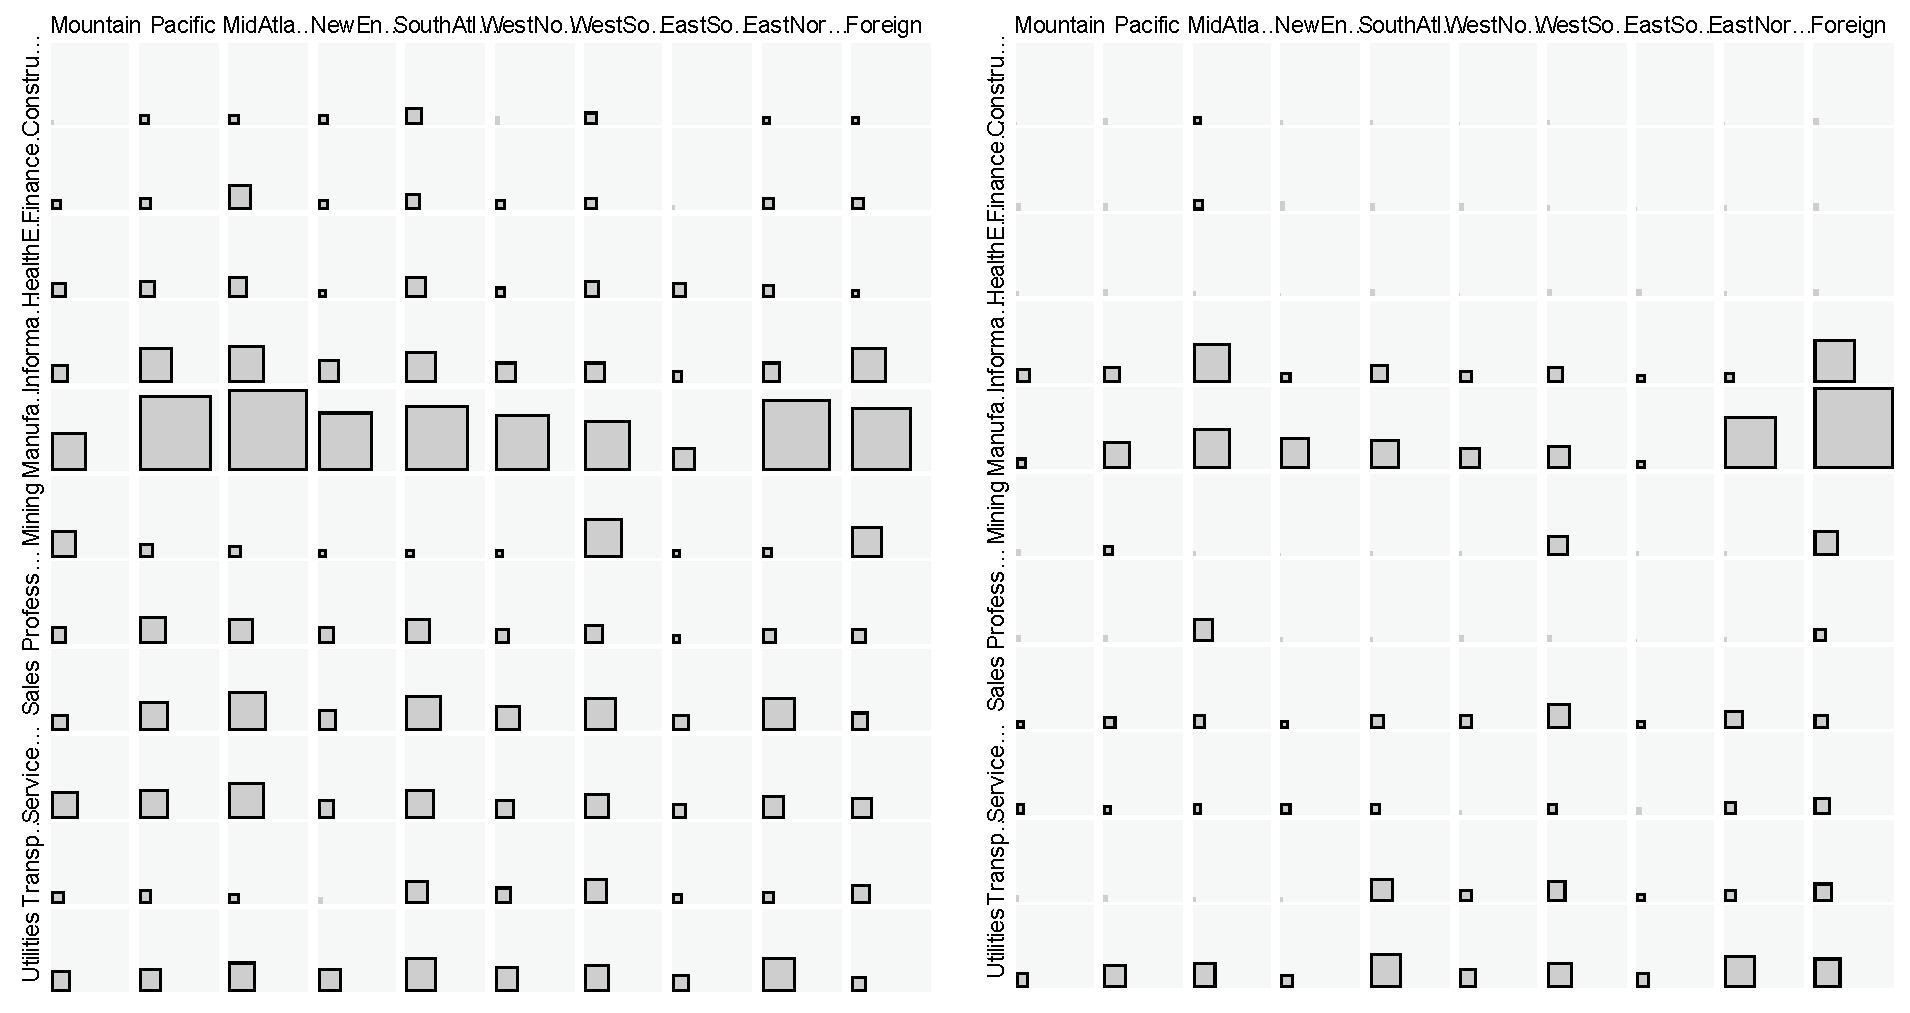
\includegraphics[width=12cm]{IndRegAndWtd.pdf}
      \caption{\label{indreg}\em Fluctuation diagrams of over $80,000$ companies by sector and region.  The plot on the left shows counts of companies and the plot on the right is weighted by the total assets of the companies.}
      \end{center}

\section{Weighting in specialist graphics}
\label{spec}

\subsection{Self-weighted histograms}
\label{shist}
Self-weighted histograms are an interesting special case of weighted graphics, where the display is weighted by the variable itself.  There was an example in Section~\ref{family}.  Note that the term self-weighting is used in survey theory differently.  In a self-weighting sample each case is given the same weight, so no weights are actually needed \citep{cochran:1954a}.

Self-weighted histograms are useful, when absolute sizes of units are to be compared rather than numbers of units.  If the distribution of turnover of different companies is plotted in a standard histogram, then each company is represented by the same column area, whether they have a huge turnover or hardly any.  A self-weighting histogram of the same data allocates an area to each company proportional to its turnover, so that the larger ones are correspondingly emphasised compared to the smaller ones.  Another application would be in displaying the distribution of the numbers of fatalities in traffic accidents.  In a self-weighting histogram, twenty accidents each with one fatality are equivalent to one accident with twenty fatalities.  In a standard histogram the more serious accidents are visually downplayed.  Figure~\ref{uvw} shows another application from a Bayesian Model Averaging study \citep{unwin:2003}.  Plotting the probabilities in an unweighted histogram does not reflect their importance.  Imagine how the unweighted and self-weighted histograms would look, if one model had an a posteriori probability of $0.65$ and the other $35$ each had one of $0.01$.  These examples are all importance weighting.

\begin{center}
      \includegraphics[width=12cm]{uvwWtdHist.pdf}
      \caption{\label{uvw}\em A self-weighted histogram of the posterior probabilities of $36$ models from a Bayesian Model Average analysis.  Bar heights are proportional to the sums of probabilities of the models in the bin.  The horizontal scale is from 0 to 0.2 with equal class widths of 0.01.   The model fitted in a non-Bayesian analysis is highlighted.}
      \end{center}
      
      When complex mosaicplots with many cells are drawn, we usually want to concentrate on the larger ones and it is helpful to know how large they are and to be able to select them.  In the software MANET \citep{unwin:1996} a histogram of cell sizes may be drawn for a mosaicplot.  The histogram is self-weighted to reflect the number of cases rather than the number of cells, cf. Figure~\ref{binmosaic} and frequency weighting is being used.


\begin{center}
      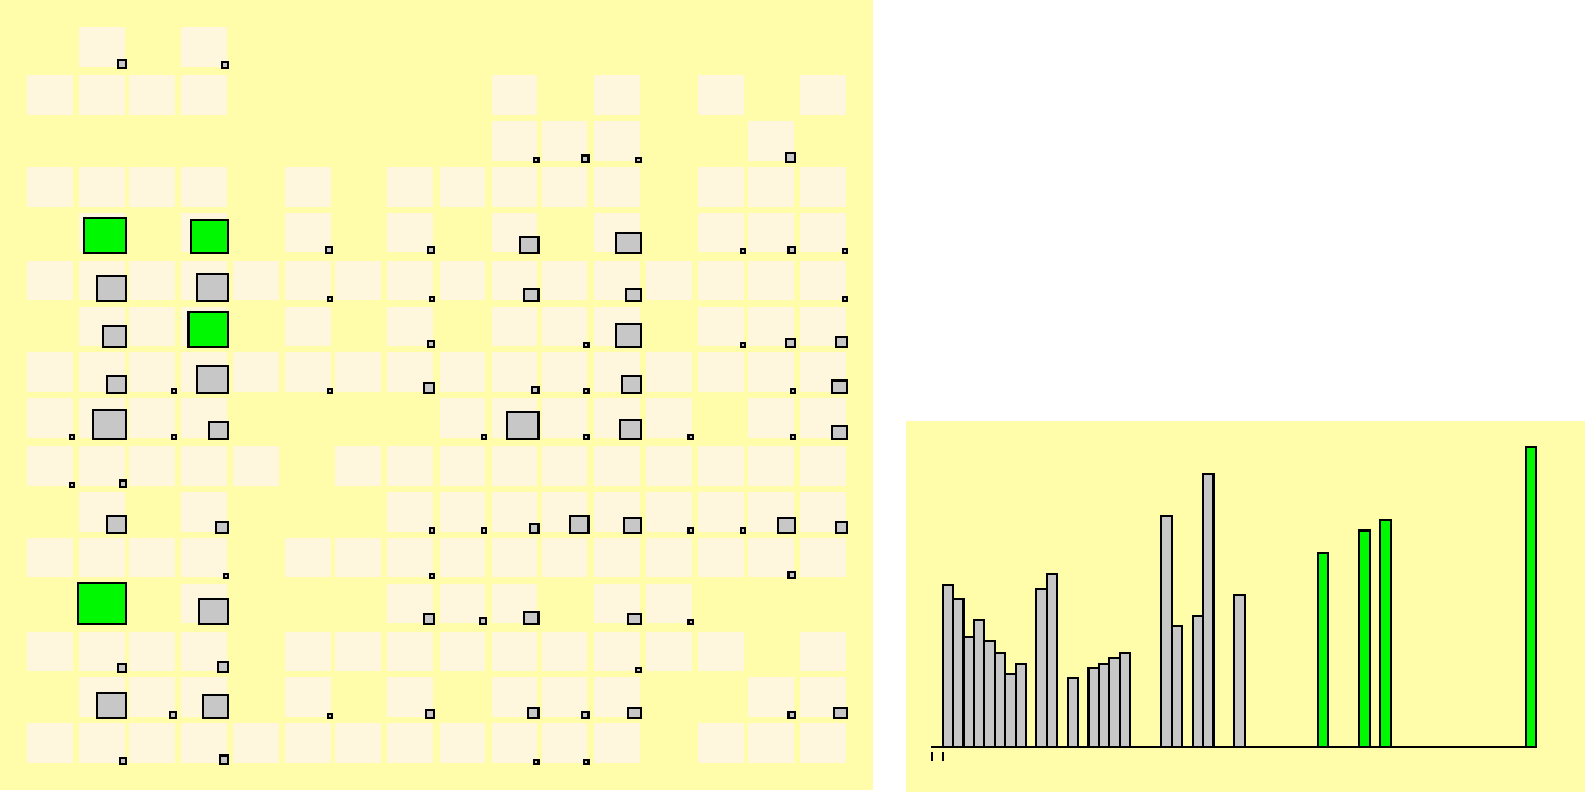
\includegraphics[width=12cm]{binmosaic.pdf}
      \caption{\label{binmosaic}\em A fluctuation diagram of the eight binary variables of the Rochdale dataset \citep{whittaker:1990}.   The accompanying histogram shows the distribution of cell sizes weighted by the sizes themselves.  The four biggest cells have been selected and contain just over $25\%$ of the data.  Linking to barcharts of the variables (not shown) reveals that they are all combinations where both husband and wife work, there is no child under $4$, no one else in the household works and the family is not Asian.}
      \end{center}

Since weights must be additive, the histogram of percentages of blacks in Section~\ref{pop} could not have been self-weighted.  Had the actual numbers of blacks in each county been plotted, then the plot could have been self-weighted.

Finally, it's worth noting that any histogram drawn of weights should really be drawn with self-weighting.  The European Social Survey, http://ess.nsd.uib.no/, publishes histograms of the design weights for each country, but not self-weighting ones.  Not all surveys report their weight distributions in full.
\newpage
\subsection{Graphics in metanalysis}
\label{meta}

\piccaption{\label{hc} An unweighted histogram of the weights for $8$ groups (above) and a self-weighted histogram of the same weights (below).  Both histograms have $12$ bins of width $0.1$, starting at $0$.}
\parpic[r]{\mbox{\includegraphics[height=7cm]{HChists.pdf}
}}

Metanalysis uses analytic weights.  How best to combine them, when they differ a lot is an interesting question.  Long before the term metanalysis ever became current, \cite{cochran:1954b} suggested adjusting weights of groups of results with low variation, and consequently high weights, upwards.  ``The method prevents an experiment which happens to have a small estimated error from dominating the result, while allowing the less precise experiments to receive lower weights.''  Cochran's approach required subjective judgement and so \cite{mosteller:1982} suggested a more objective approach.  Plotting the weights would have helped.  Figure~\ref{hc} shows the weights from the eight different sets of gravity measurements used by \cite{mosteller:1982} to illustrate their approach.  The lower plot demonstrates clearly why adjustments are necessary.  (Though a more reasonable conclusion might be that the experiments are simply not comparable.  The groups included from $8$ to $13$ measurements, so that the differences in weights were primarily due to the variances being very different.)

Comparable results from many different studies are often displayed in a forest plot of parallel confidence intervals.  As mentioned in Section~\ref{aw}, this means that studies with low weight take up more visual space.  An alternative taking up less space would be to use a dotplot, with dotsize a function of the analytic weight.  A combination of the two might also be effective.

Funnel plots are used to illustrate possible publication censoring through lack of significance.  Implicitly, the studies displayed at the top of the funnel have higher weight, mainly because they are larger.  It would be easy to make this explicit by drawing the points with pointsize a function of the weight.

\subsection{Edges and flows}
\label{edge}
Weighting arises naturally in displaying geographic flows or other graph structures.  Flow sizes such as trade flows \citep{unwin:1992}) or traffic flows may be represented crudely by the width of the links.  The same may be applied to the edges of network graphs, though colour or transparency with anti-aliasing are possible alternatives \citep{wills:2006}.  Figure~\ref{traffic} shows traffic flows in the centre of Augsburg in 2001.   Like any modern city, Augsburg has encouraged traffic to avoid the city centre and this reflects the patterns observed.  North-South traffic avoids the centre altogether.

\begin{center}
      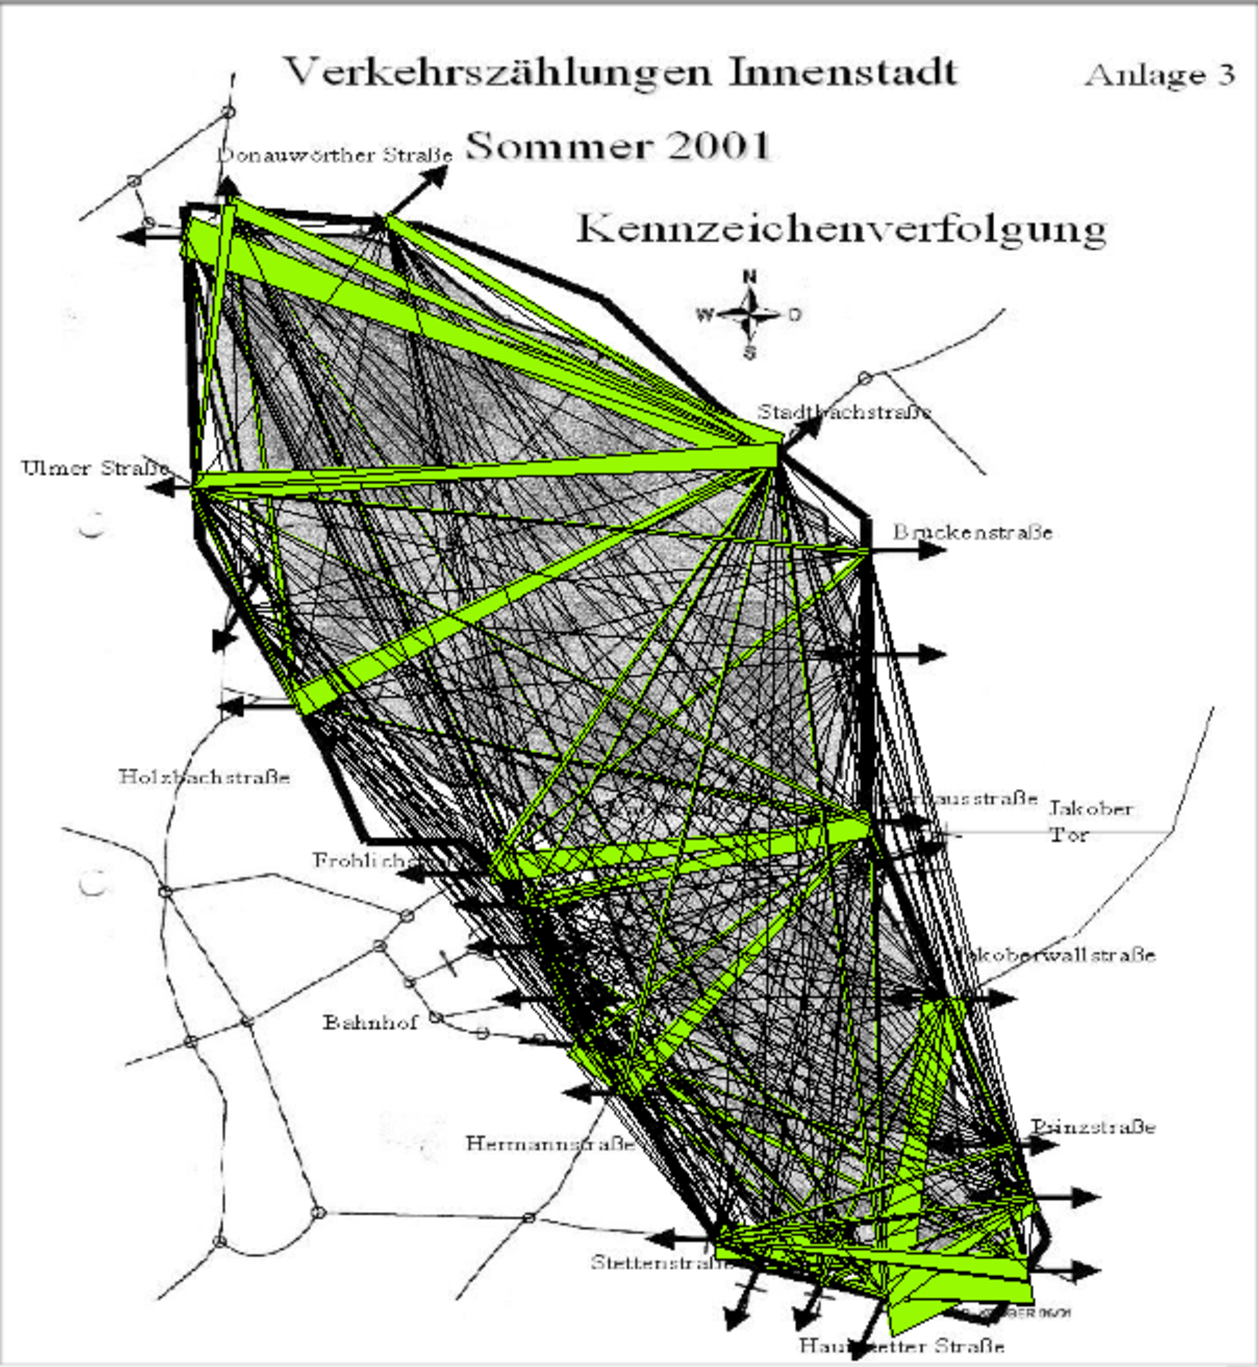
\includegraphics[width=12cm]{TraffFlow.pdf}
      \caption{\label{traffic}\em Traffic flows in the centre of Augsburg in 2001. The flows are drawn as wedges with the base proportional to the amount of traffic. }
      \end{center}

\section{Software}
\label{sw}
Standard statistical software packages do not tend to offer weighted options for plots.  As remarked in Section~\ref{intro}, this is not essential as some of the displays can be achieved by a restructuring of the dataset --- however, it does provide more flexibility and ease of use.  Both the interactive graphics packages Heike Hofmann's MANET \citep{hofmann:2000a} and Martin Theus's Mondrian \citep{theus:2005} offer weighting for all area plots and MANET has bubbleplots as well.  Amongst R packages, Thomas Lumley's survey package offers weighted histograms and boxplots, and bubbleplots and hexagonal binning for weighting scatterplots.  Survey only works with sampling weights.  Hadley Wickham's ggplot package for R is more general and offers a range of weighted static plots and any kind of weighting can be used.

\section{Conclusions}
\label{conc}
Weighted graphics are a valuable supplement to standard statistical graphics.  They display different aspects of datasets and enable additional insights to be gained.  Weighting is particularly useful for area plots and its use is enhanced for exploratory analyses by incorporating interactive tools, as is true for all graphics.

The interpretation of a weighted graphic depends on the variable or variables displayed, on the type of weighting involved, and, if importance weighting is used, on the weighting variable.  As with all components of statistical analyses, care must be taken in interpreting the results.

\bibliographystyle{dcu}
\bibliography{Wts}


\end{document}